%This is the section: RTPC Expert of the RTPC Operations Manual

\subsection{Subsystem Expert Resposibilities}
The RTPC system expert have following responsibilities:

\begin{enumerate}
	\item Complete hot checkout sign-off before the start of the rg-f run period (sub-section \ref{sub-sec:hotcheckout} )
	\item Respond to calls on the on-call phone to resolve issues with the BONuS/RTPC during data taking (sub-section \ref{sub-sec:onCallRespose})
	\item Monitoring and control of the BONuS gas system (sub-section \ref{sub-sec:gas_control})
	\item Adjust the system HV settings (sub-section \ref{sub-sec:HVsetting})
	\item Monitoring and control of low voltage (sub-section \ref{sub-sec:LV_control})
	\item Monitoring BONuS Interlocks and the RTPC system performances (sub-section \ref{sub-sec:PerfomanceMonitor})
	%\item Monitoring and control of the DMS (sub-section \ref{sub-sec:DMS})
	\item Make repairs to the hardware during maintenance periods (sub-section \ref{sub-sec:maintainance})
	\item Perform pedestal run for data taking (sub-section \ref{sub-sec:ped})
\end{enumerate}


\subsection{Hot Checkout}
\label{sub-sec:hotcheckout}

Prior to the start of each beam running period, each subsystem Group Leader is responsible to review the components of their systems to be sure that they are fully operational. This review is referred to as “hot checkout”. The hot check-out is an online checklist for each subsystem that includes a sign-off for all hardware elements of the system (e.g. HV, LV, gas). Before the RG-F run period, the hot checkout of the RTPC (BONuS) sub-system should be performed which includes the verification that the detector is operational, and the Slow Controls system for the Gas, HV and LV is functioning. Figure \ref{fig:hco} shows the expansion of the Hot Chekout list for the RTPC (BONuS), including different sub-system of the Hall B.

\begin{figure}[H]
	\centering
	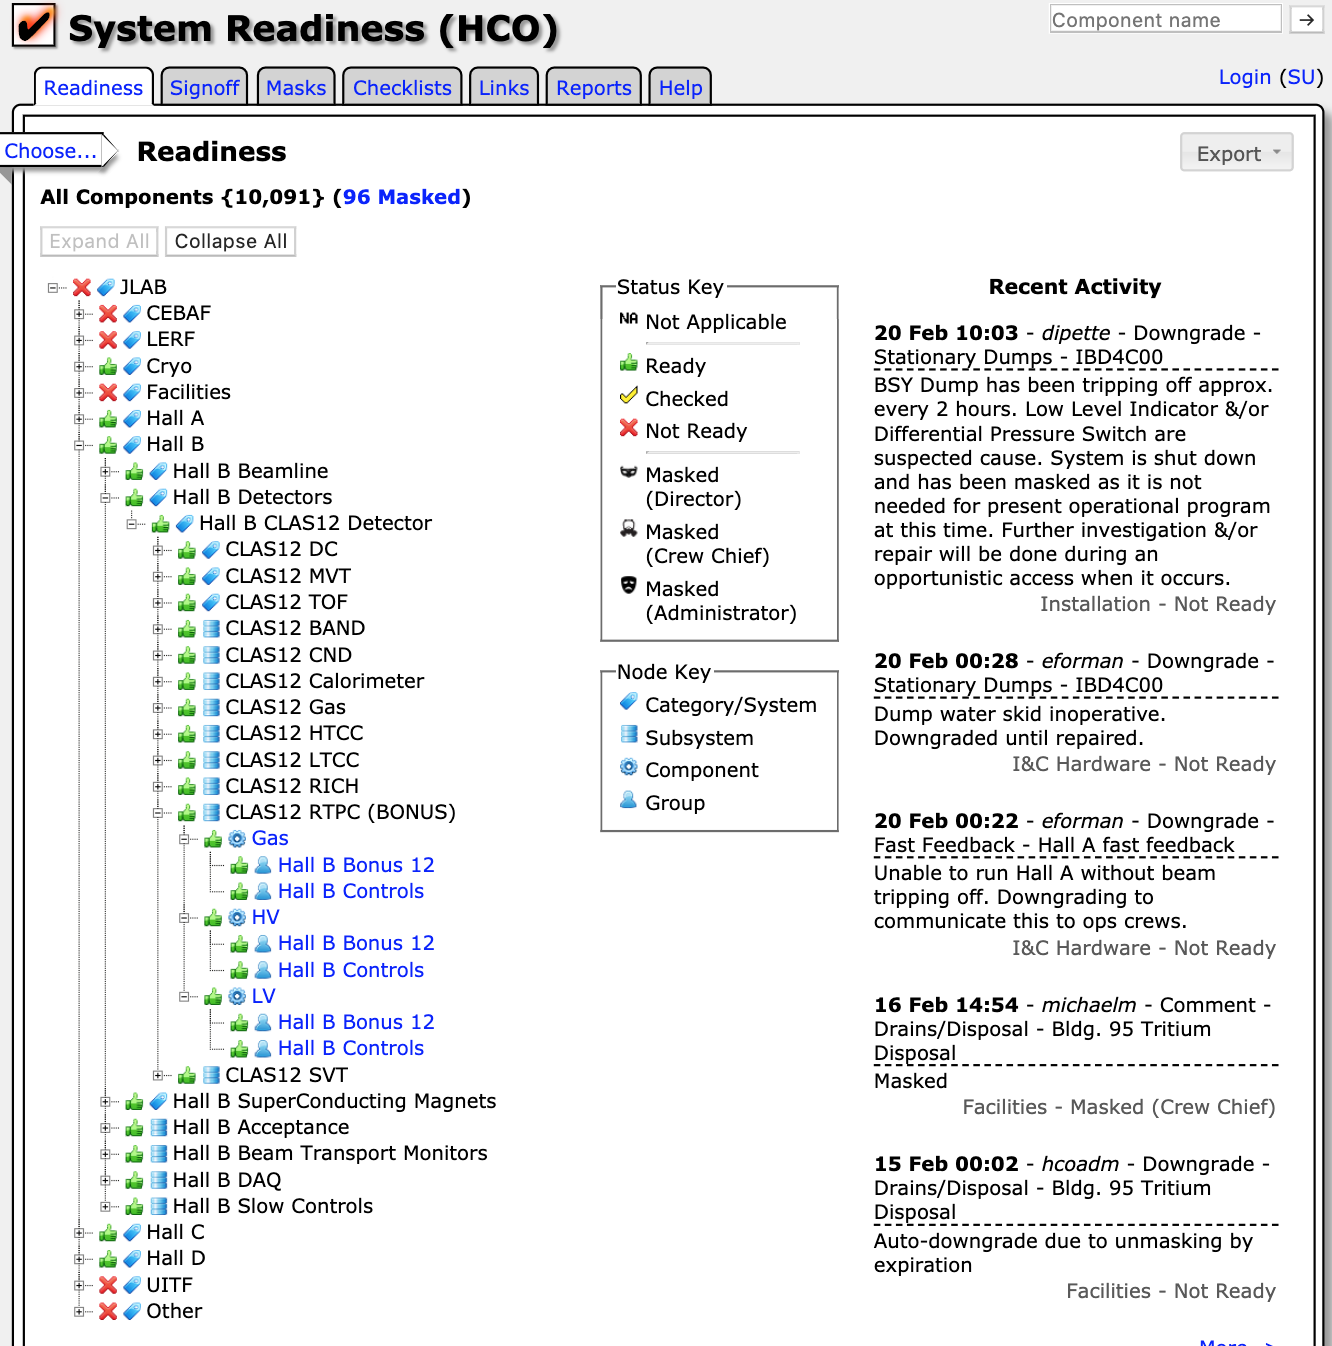
\includegraphics[height=13cm,width=13.5cm]{HCO}
	\caption{Hot-checkout List of Hall B}
	\label{fig:hco}
\end{figure}


\subsection{On-Call Responsibilities}
\label{sub-sec:onCallRespose}

Each subsystem Group Leader will organize a list of on-call experts who will take responsibility for carrying a cell phone to allow 24 hour access to experts who can address any problems that arise during a beam running period. The phone numbers of all subsystem experts are posted on the run page \cite{runpage}. Any problems that cannot be quickly solved by the shift workers, where quickly amounts to 10 to 15 minutes, should result in a call to the relevant expert cell phone. The RTPC on-call phone number is {\color{red}757-329-4844}.

The on-call experts can often diagnose problems over the telephone, but there are times when they will have to go to the Counting House to more fully address an issue. One of the important responsibilities of the on-call experts is to share all issues that they cannot resolve with the RTPC subsystem group periodically and help to make practical decisions regarding which problems that require access to Hall B for immediate attention and which can be delayed to periods when the accelerator is down or other work is scheduled in the hall.

\subsection{BONuS Gas system}
\label{sub-sec:gas_control}

BONuS gas sytem is divided into two categories: i) Drift gas and ii) Target gas. Both of these gas sub-system have separate EPICS GUI monitoring as shown in figure \ref{fig:gas_monitoring} and figure \ref{fig:target_gas}. Details of the different parameters used in these GUI is found in the document attached in the Appendix (page \pageref{appedix}).

\begin{figure}[H]
	\centering
	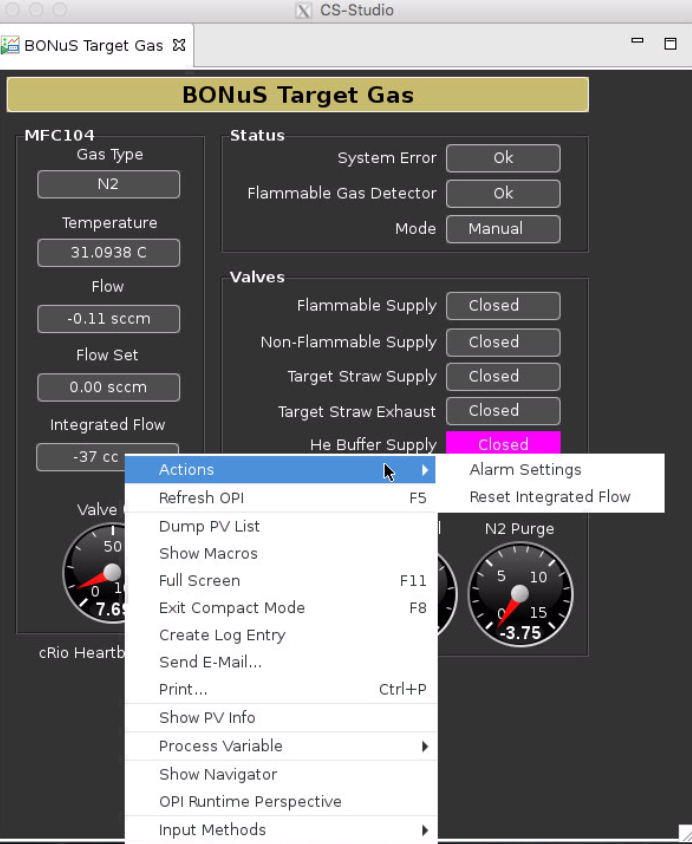
\includegraphics[height=10cm,width=10cm]{target_gas1}
	\caption{Target gas monitoring GUI}
	\label{fig:target_gas}
\end{figure}

In both the monitoring, expert also cannot change current value of any variables, except integrated flow. When you right click on the integrated flow, you will have options as shown in figure \ref{fig:target_gas}. Click on: action-> Reset intergrated flow to reset the total gas consumption after using a bottle of drift/target gas. Alarm can be activated to get alert for changing the gas bottles.

All the gas controls is performed from a windows pc at counting house (first computer on the right jafter entering into Hall B counting house). Use your Jlab username and password to open the pc, and enter GUI.vi in the search option at the bottom of the desktop. When you click on GUI.vi, it will open a Lab-view window as shown in figure \ref{fig:rtpc_gas_control} or \ref{fig:target_gas_control}. Control on the BONuS drift gas is detailed in the Appendix (page \pageref{appedix}).

\begin{figure}[H]
	\centering
	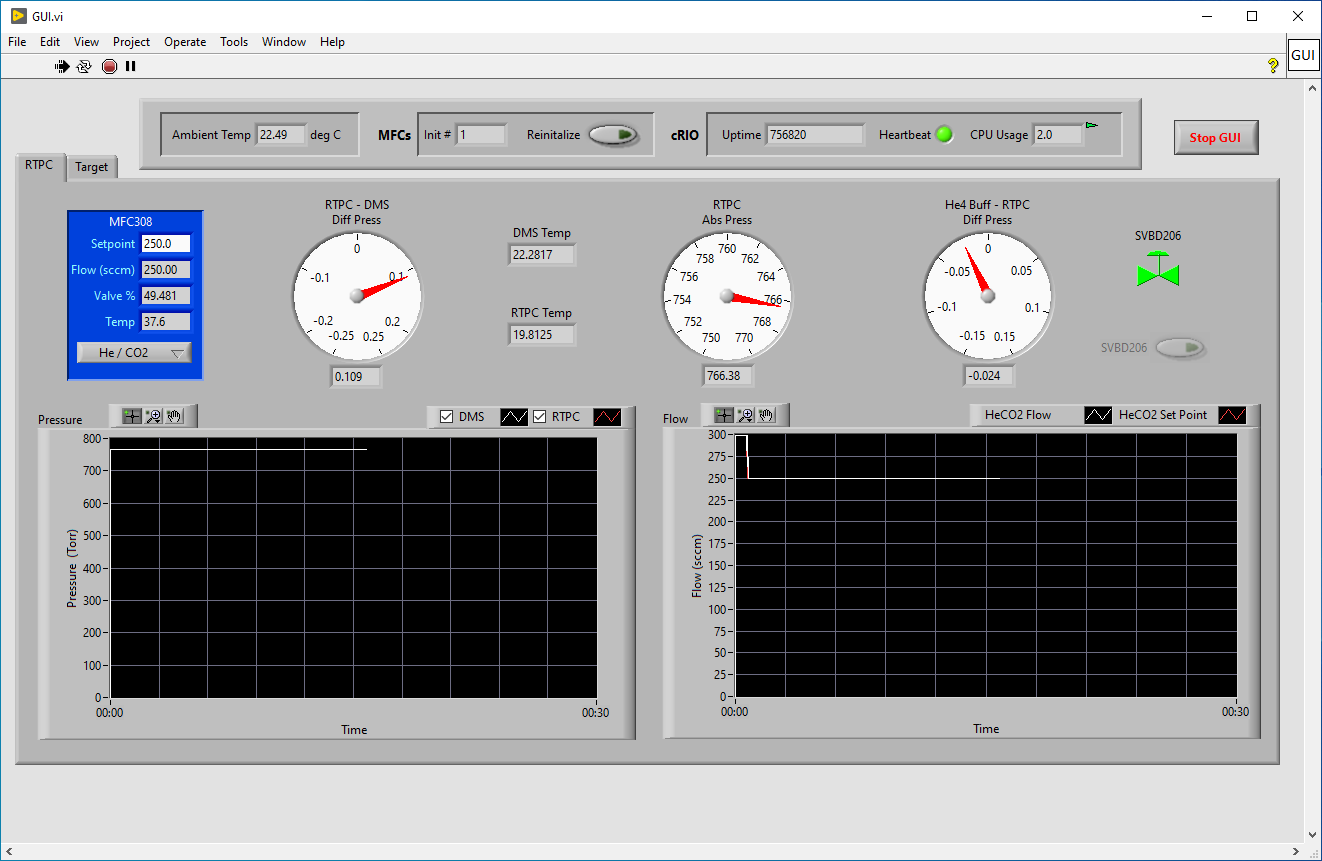
\includegraphics[height=9cm,width=13.5cm]{RTPC_gas_control}
	\caption{RTPC gas control from Lab-view Interface}
	\label{fig:rtpc_gas_control}
\end{figure}


\begin{figure}[H]
	\centering
	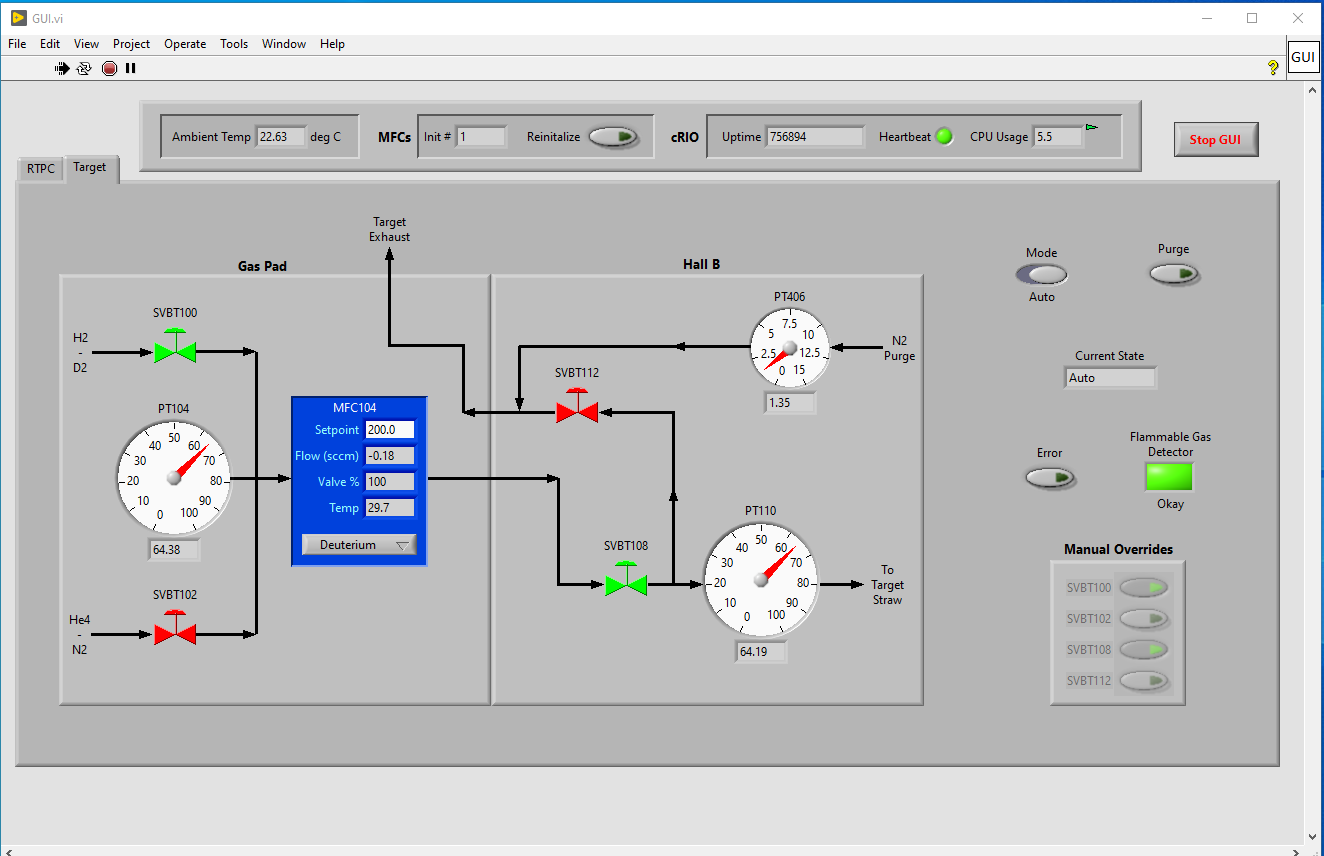
\includegraphics[height=9cm,width=13.5cm]{target_gas_control}
	\caption{Target gas control from Lab-view Interface}
	\label{fig:target_gas_control}
\end{figure}

Details of BONuS target gas control is explained in \href{https://wiki.jlab.org/clas12-run/images/a/ac/BONuS_Target_Gas_System_Manual.pdf}{Target Manual}, so please look at that document before starting to control the target gas.\\

There is also BONuS HV interlock related with both gas system (2 related to target gas and 5 related to drift gas as shown in figure \ref{fig:interlock}), so please make sure that which interlock will be active before using the gas controls. Mostly bypass the target related interlock before purging the target gas. Please, don't bypass any interlock  during the data taking. If it's absolutely necessary to bypass any, inform all the RTPC expert group and also put log-entry in \href{https://logbooks.jlab.org/book/hbrtpc}{HBRTPC}.

\begin{figure}[H]
	\centering
	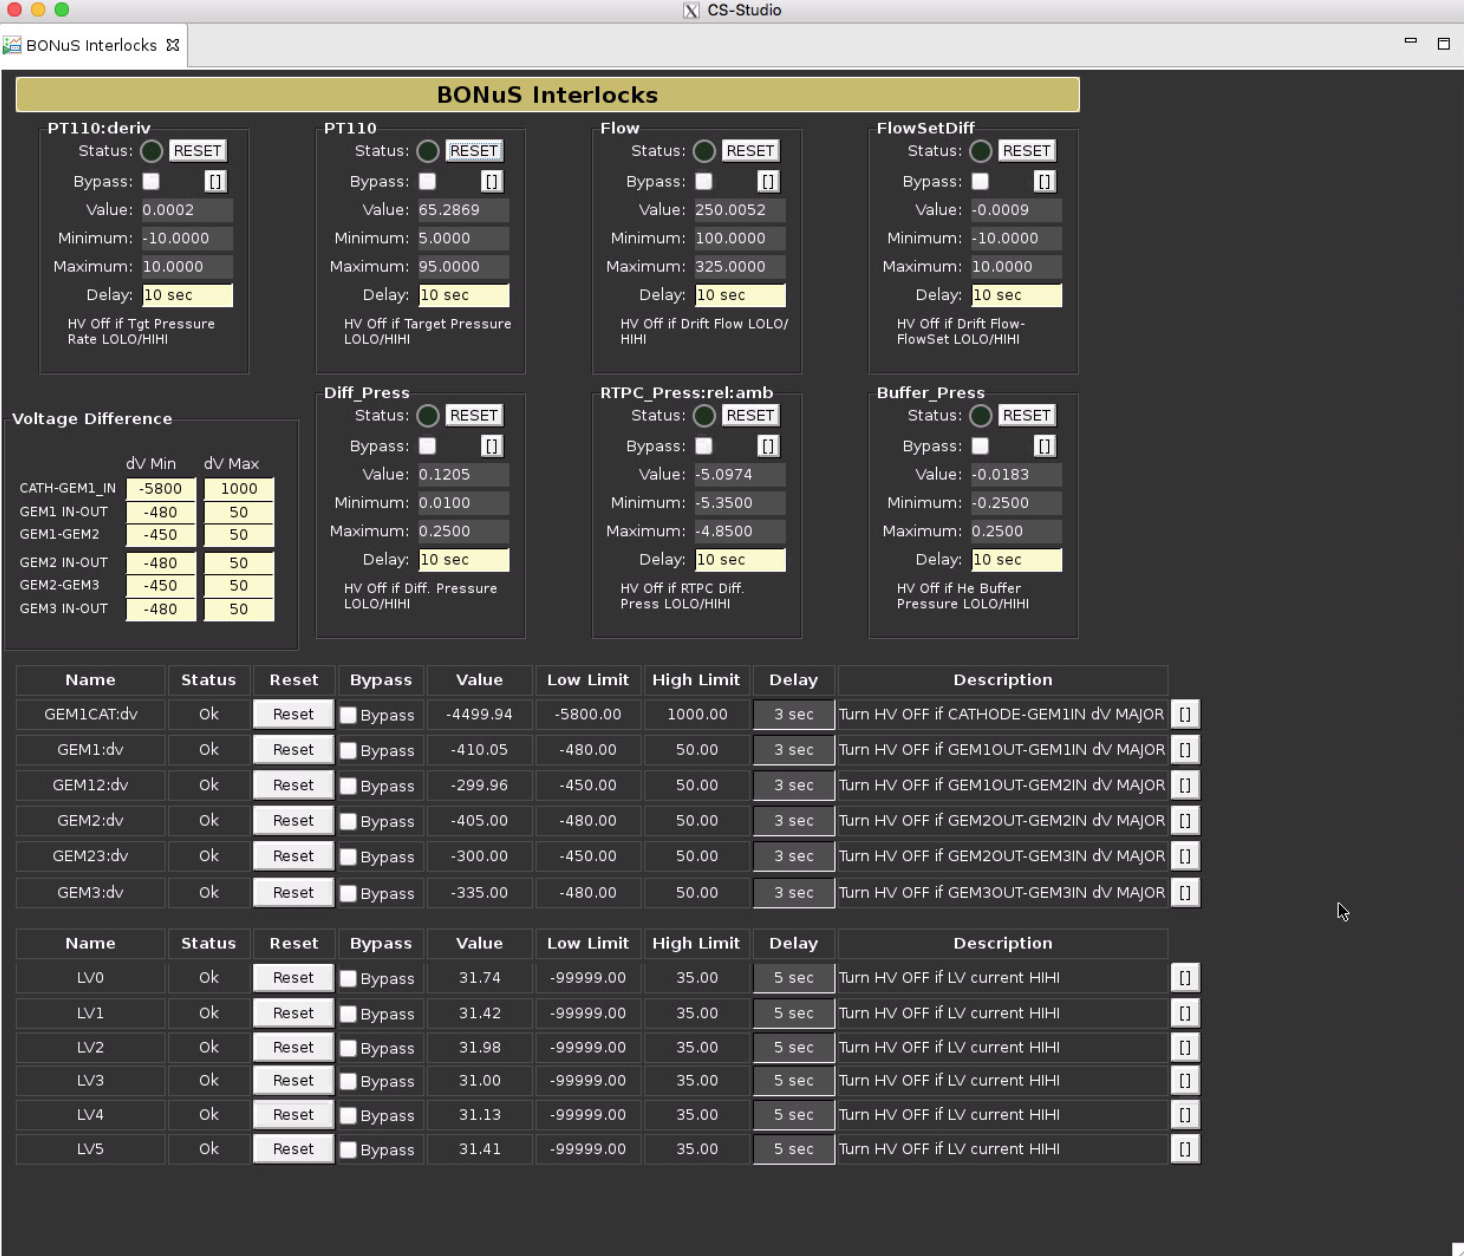
\includegraphics[width=13.5cm]{interlock}
	\caption{RTPC interlocks}
	\label{fig:interlock}
\end{figure}

\subsection{RTPC System HV setting}
\label{sub-sec:HVsetting}
Expert Interface has access to change several parameters in the RTPC HV control. Along with the ``All HV ON" and ``All HV OFF" from menu, individual channel can be cotrolled. This interface also has control over voltage setting, trip current setting, trip delay setting and also the setting for the ramping rate. Voltage and current limit for each channel can be set directly from the interface by typing new values in the respective boxes of `Vset' and `Iset' as shown in figure \ref{fig:hv_expert1}. This interface also shows the HV sequence timing for ramping up high voltage included in ``All HV On" for both Novice and Expert mode.
\iffalse
\begin{figure}[H]
	\centering
	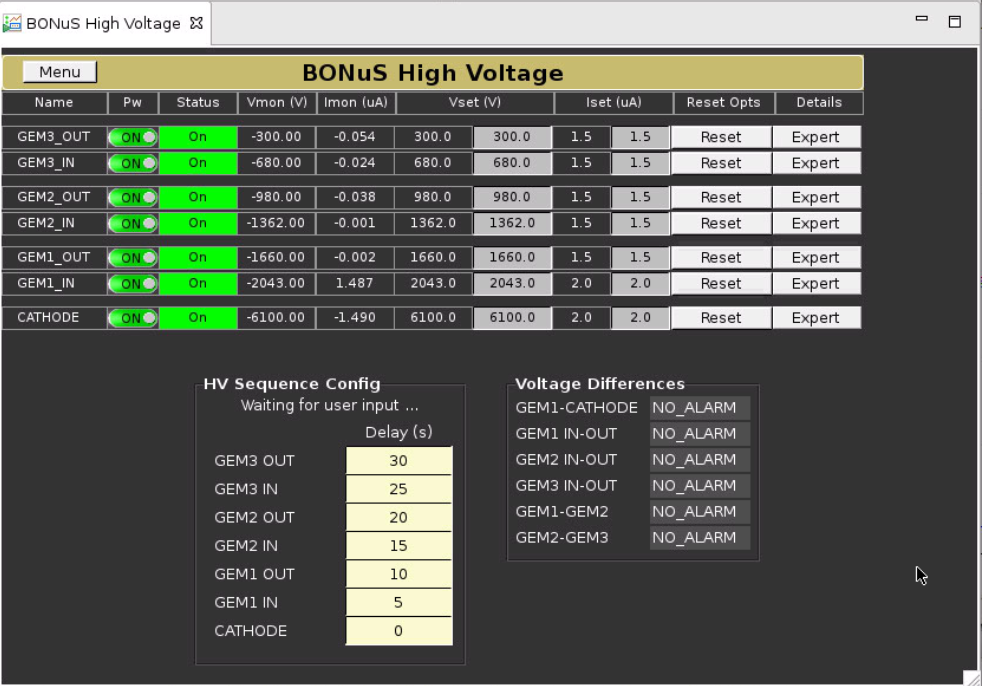
\includegraphics[width=13.5cm]{hv_expert0}
	\caption{RTPC HV control Interface for Expert}
	\label{fig:hv_expert0}
\end{figure}
\fi
\begin{figure}[H]
	\centering
	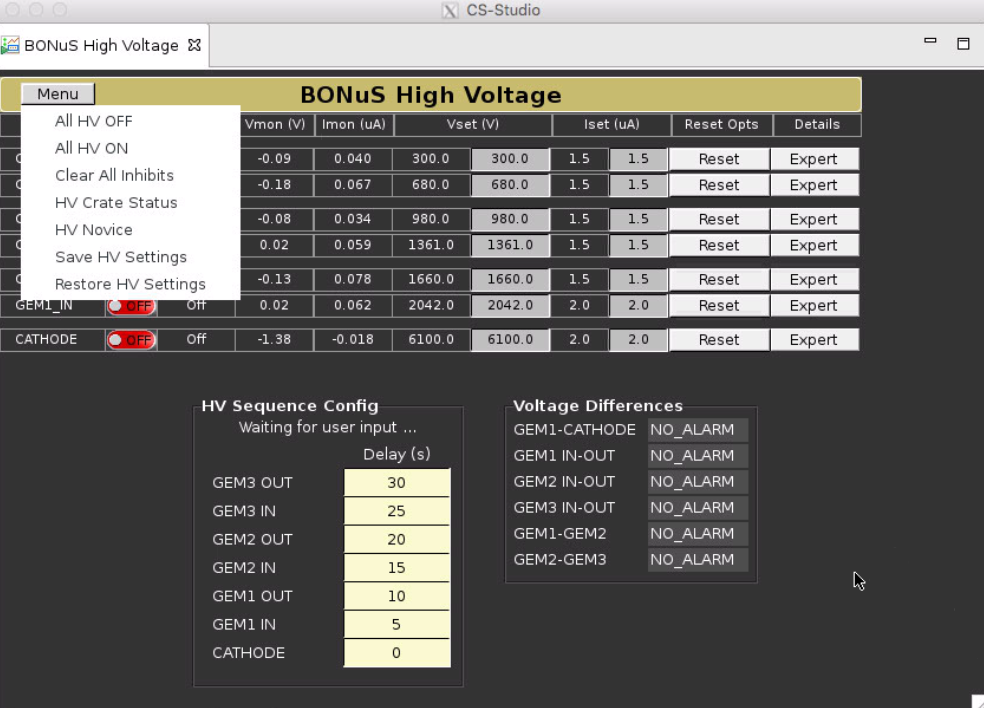
\includegraphics[width=13.5cm]{hv_expert1}
	\caption{RTPC Expert HV control Interface}
	\label{fig:hv_expert1}
\end{figure}

There is no need to clear any error on channels while using ``All HV On" as clear is embeded within it. However, while using individual channels ``Clear All Inhibits" is used to clear any errors occured in any channels. Clearing the error on chanels can be done by clicking on ``Reset--$>$clear" on that channel.\\

Different HV setting for RTPC related with different runs (Prodution, cosmic) are saved which could be restored by clicking ``Restore HV Setting" on the menu. This helps to reduce errors of typing numbers in the GUI and also restore the previous setting after change.\\

Ramping rate and the trip time can not be set from this interface. To change these, click on the expert on the particular channel which gives a new window as shown in figure \ref{fig:expert_hv}. In this expert screen, ramping rate and trip time are inside controls box (Lower left) which can be changed typing new number in the corresponding box. Both ramping up and down rate will be set for all the GEM-related channels when changed in one of them. For cathode, these are independent of GEM chanels.

\begin{figure}[H]
	\centering
	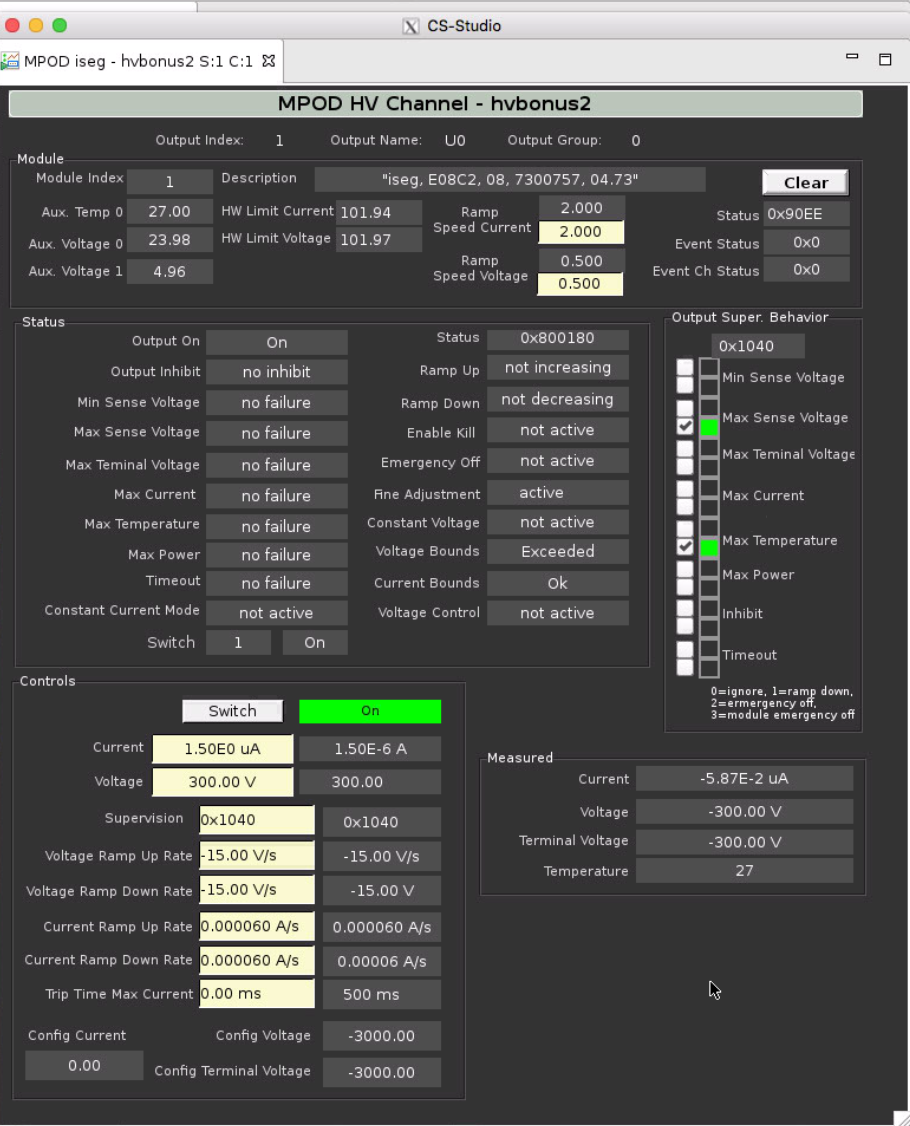
\includegraphics[width=13.5cm]{expert_hv}
	\caption{HV channel control for experts}
	\label{fig:expert_hv}
\end{figure}

If the Mpod crate has issues, `output failure', `input failure' or `crate status' alarms will appear. If so, use ``HV Crate Status" under menu of figure \ref{fig:hv_expert1} to get the crate status GUI. This GUI shown in figure \ref{fig:hv_crate} allows users to remotely reboot (ON/OFF) the crate to clear all the errors. This is only done, if there is issue with both the power supply modules or as a last resort to fix unknown issue related to the power supply.
\begin{figure}[H]
	\centering
	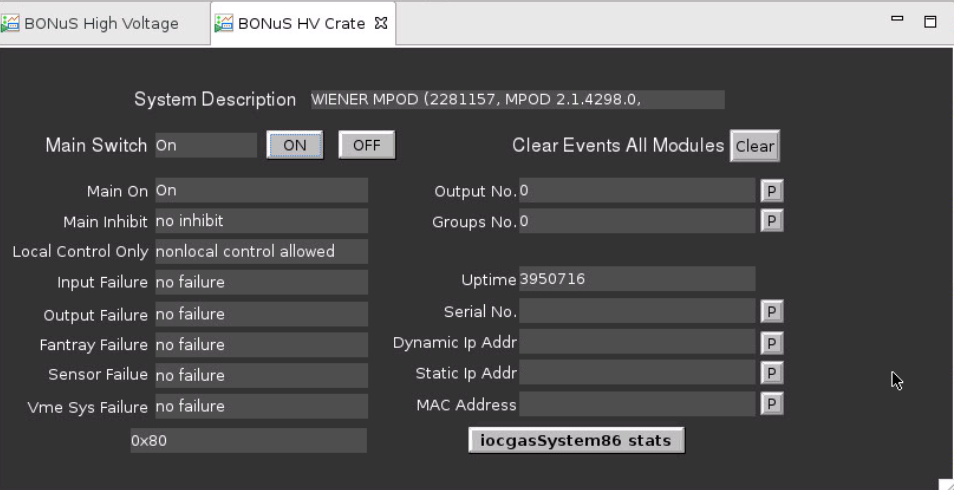
\includegraphics[width=12cm]{hv_crate}
	\caption{RTPC HV crate status}
	\label{fig:hv_crate}
\end{figure}

\subsection{Monitoring and Control of LV}
\label{sub-sec:LV_control}

Low voltage is applied to the FEUs for the Readout of the RTPC detector. There are six crates for the total 48 FEUs, with 8 FEUs in each crate. Among 8 FEUs in each crate, 6 are used by RTPC and one by FMT. If there is any communication errors related with FEUs, LV might need to turn ON and OFF. While doing this, both FMT and RTPC are affected. Each individual crate can be turned On and OFF as well as all the crates at once, but before doing so it needs to figure out which FEU has issue and which cart it belongs to. Turning All OFF and On of LV can be done from the RTPC overview GUI (fig. \ref{fig:overview}). But to turn OFF/ON individual crate, LV controls GUI (as shown in figure \ref{fig:LV})is needed which is obtained by clicking on the ``parenthesis--$>$LV control" near the Low Voltage in the RTPC overview GUI (fig. \ref{fig:overview}).

\begin{figure}[H]
	\centering
	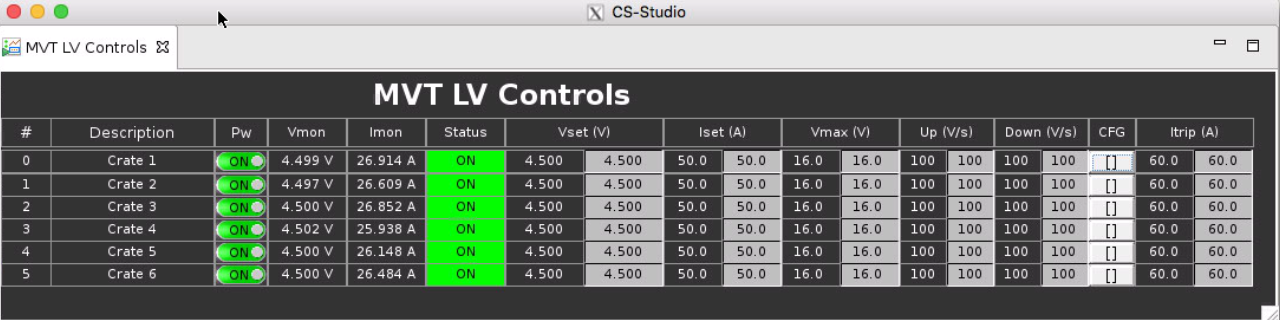
\includegraphics[height=4cm, width=13.5cm]{LV}
	\caption{LV controls on EPICS Interface}
	\label{fig:LV}
\end{figure}
 {\color{red} Note:} RTPC HV and FMT HV interlocks might be active during power cycle of the LV for FEUs if it takes longer to power up FEUs. Currently, delay setting is 5sec. We can set max delay of 10 sec. To go higher than this, Saclay group should be consulted. 

\subsection{Monitoring BONuS Interlocks and the RTPC System Performances}
\label{sub-sec:PerfomanceMonitor}

BONuS interlock for High voltage are related with target gas, drift gas, LV and GEM biasing voltages as shown in figure \ref{fig:interlock}. The minimum and maximum value at the interlock setting could not be set from Interlock GUI. These maximum and minimum values are actually set from the Alarm setting of particular PVs in the respective sub-system GUI. One example is shown in figure \ref{fig:alarm_limit} for the MFC flow rate of drift gas, which is obtained by double clicking the PV value on Drift gas GUI as shown in figure \ref{fig:gas_monitoring}. Setting LOLO and HIHI in the alarm setting also set the max and min of Interlock.

\begin{figure}[H]
	\centering
	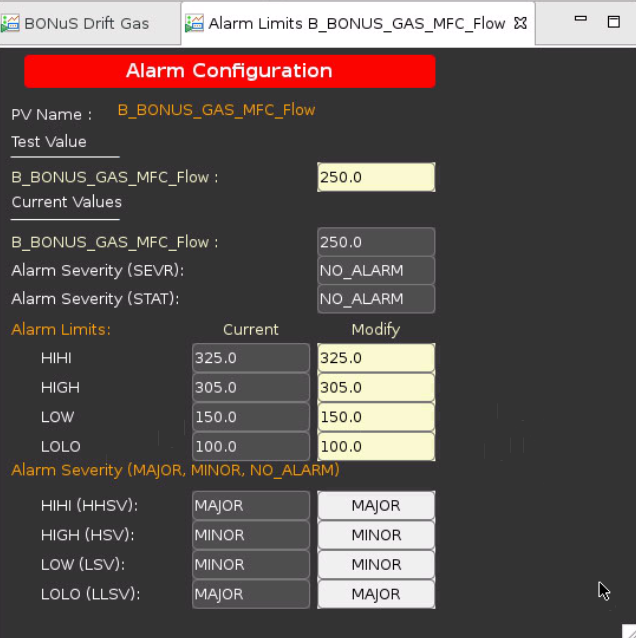
\includegraphics[height=9cm,width=9cm]{alarm}
	\caption{Alarm Limit settings}
	\label{fig:alarm_limit}
\end{figure}

Monitoring the strip charts of all the PVs periodically and also uploading them in \href{https://logbooks.jlab.org/book/hbrtpc}{HBRTPC} is crucial. Adjusting the parameters accordingly for the better performance of the RTPC is an important task of the RTPC experts.

\subsection{Monitoring and Control of the DMS}
\label{sub-sec:DMS}

DMS is run from dedicated vncserver on clondaq4:1 (DMS\_BONUS). To access the vncserver follow the following steps:\\

i) From Hall network (from any clonpc computers):
\begin{center}
	\centering \textbf{vncviewer clondaq4:1 -RemoteResize=0 -Shared}
\end{center}

ii) From personal computer with hallgateway following steps should be completed:

\begin{center}
	\centering \textbf{ssh -Y username@login.jlab.org}\\
	\centering \textbf{ssh -Y username@hallgw}\\
	\centering \textbf{ssh -Y clasrun@clonsl2}\\
	\centering \textbf{vncviewer clondaq4:1 -RemoteResize=0 -Shared}
\end{center} 

Being in the vncserver, dms daq computer is accessed using 'ssh -Y daq@bonusdms'. High voltage supply GUI is opened using command 'sudo CAENGECO2020'.

\subsection{Maintainance of the RTPC System}
\label{sub-sec:maintainance}

RTPC experts are also responsible for any change/maintainace of the RTPC system. Mostly the high voltage and the gas panel and control could be the issue. After the decision of the RTPC experts, maintainance of the RTPC sub-system is performed either accessing the hall or from the counting house. Every maintainance should be logged in \href{https://logbooks.jlab.org/book/hblog}{HBLOG} and \href{https://logbooks.jlab.org/book/hbrtpc}{HBRTPC} logbook.

\subsection{Pedestal Run and configuration test}
\label{sub-sec:ped}

RTPC data are collected by FEU and only the ADC samples above threshold (specified by BONuS group) are written in output. Common mode noise rejection and pedestal subtraction is also performed by FEU containing DREAM chips. To apply those constains, configuation of the RTPC DAQ should have access to pedestal file and the threshold files. So, the first step is to take pedestals of the our system. After powering up both FEU and BEU, we need to be sure that our DAQ system is synchronised and working correctly.

To take pedestals, go to $\sim$/mvt/Codascript/ directory form any clon-machines in the counting house and use the following command in terminal:

\begin{center}
	\centering \textbf{MvtRunBatchCol\_HR PEDRUN ./mvt2crates\_bonus 500 DEBUG}
\end{center}

Before entering the command, make sure that nothing is running on mvt1 and mvt2 crates. Mostly, no data taking nor even prestart is running from CODA.

The above command open up two new windows (one for mvt1 and other for mvt2) and takes the pedestal of our electronics using `mvt2crates\_bonus.cnf' configuration file for FEUs, produced pedestal file and ZS threshold file to be used in the data taking. But, the above command doesn't take number of samples mentioned in config file, but takes fixed 16 samples for the pedestal run. During pedestal run with the above command, events are collected with 50KHz internal trigger.

Their are chain of processed included in this command which takes pedestal data, analyze the data for average pedestal and noise, perform common mode noise rejection, calculate zero suppression ADC values for all channels based on provided threshold value and the noise, modifies threshold and put mask to individual channels mentioned in MvtMask.txt file, creates the pedestal file and final threshold file for FEUs, and also creates and transfers the final configuration file of the mvt1 and mvt2 to the destination for the CODA run.

During pedestal run main window and two new windows are running. After completion, main window shows pedestal run is done. But new xterm windows shoud be closed manually. If pedestal run is running for 15 minutes and still not finished, please contact expert.

{\color{red}Note:} If you have any issues taking pedestal in mvt1 or mvt2 crates for BONuS, please contact \href{mailto:jpoud001@odu.edu}{\color{blue}\nolinkurl{Jiwan Poudel}}. As we have large window of 80 samples and also sparse readout, we are not using MvtRunBatchCol to take pedestals.

If you didn't see pedestal noise plot, use the following command:

\begin{center}
	\centering \textbf{xmgrace -p GraceNoise\_mvt1.par -autoscale y  filename}
\end{center}

Filename should have .ace extention.\\


{\large[}{\color{red} Note:} For the cosmic test with mvt1, mvt2 (BONuS) and mvt3 (FMT) crates in the hall, two master configurations are available: mvt123\_ctof\_cnd\_ts and MVT123\_CTOF\_CND. While running mvt123\_ctof\_cnd\_ts configuration, data files are saved in /work/bonus/ with name tag bonustest\_. And, running MVT123\_CTOF\_CND config, data files are saved to the directory as it is run with PROD66 configuration and later sent to tape. The name of the directory would be mvt123 in /cache/. Furthermore, there are two other configurations: mvt1\_er and mvt2\_er to test the mvt1 and mvt2 separately. In all the configurations, trigger used for the cosmic test at Hall is /CTOF\_HTCC/ctof\_ts\_cosmic.trg. {\large]}
